\documentclass{acm_proc_article-sp}
\usepackage{epstopdf}
\usepackage{etoolbox}
\usepackage{listings}

\usepackage{multirow}
\usepackage{subfigure}
\usepackage{float}
\usepackage[hyphens]{url}
\usepackage{color}
\lstset{ %
language={[x86masm]Assembler},                % choose the language of the code
basicstyle=\footnotesize,       % the size of the fonts that are used for the code
numbers=left,                   % where to put the line-numbers
numberstyle=\footnotesize,      % the size of the fonts that are used for the line-numbers
stepnumber=1,                   % the step between two line-numbers. If it is 1 each line will be numbered
numbersep=5pt,                  % how far the line-numbers are from the code
backgroundcolor=\color{white},  % choose the background color. You must add \usepackage{color}
showspaces=false,               % show spaces adding particular underscores
showstringspaces=false,         % underline spaces within strings
showtabs=false,                 % show tabs within strings adding particular underscores
frame=single,           % adds a frame around the code
tabsize=2,          % sets default tabsize to 2 spaces
captionpos=b,           % sets the caption-position to bottom
breaklines=true,        % sets automatic line breaking
breakatwhitespace=false,    % sets if automatic breaks should only happen at whitespace
escapeinside={\%*}{*)}          % if you want to add a comment within your code
}

\makeatletter
\patchcmd{\maketitle}{\@copyrightspace}{}{}{}
\makeatother


\begin{document}

\title{COS 597D Project - Mobile vs Traditional Web Tracking\\(FourthPartyMobile)}
%
% You need the command \numberofauthors to handle the 'placement
% and alignment' of the authors beneath the title.
%
% For aesthetic reasons, we recommend 'three authors at a time'
% i.e. three 'name/affiliation blocks' be placed beneath the title.
%
% NOTE: You are NOT restricted in how many 'rows' of
% "name/affiliations" may appear. We just ask that you restrict
% the number of 'columns' to three.
%
% Because of the available 'opening page real-estate'
% we ask you to refrain from putting more than six authors
% (two rows with three columns) beneath the article title.
% More than six makes the first-page appear very cluttered indeed.
%
% Use the \alignauthor commands to handle the names
% and affiliations for an 'aesthetic maximum' of six authors.
% Add names, affiliations, addresses for
% the seventh etc. author(s) as the argument for the
% \additionalauthors command.
% These 'additional authors' will be output/set for you
% without further effort on your part as the last section in
% the body of your article BEFORE References or any Appendices.

\numberofauthors{1} %  in this sample file, there are a *total*
% of EIGHT authors. SIX appear on the 'first-page' (for formatting
% reasons) and the remaining two appear in the \additionalauthors section.
%
\author{
% You can go ahead and credit any number of authors here,
% e.g. one 'row of three' or two rows (consisting of one row of three
% and a second row of one, two or three).
%
% The command \alignauthor (no curly braces needed) should
% precede each author name, affiliation/snail-mail address and
% e-mail address. Additionally, tag each line of
% affiliation/address with \affaddr, and tag the
% e-mail address with \email.
%
% 1st. author
\alignauthor
Marcela Melara, Christian Eubank and Diego Perez Botero \\ 
       \email{\{melara, cge, diegop\}@princeton.edu}
}

\maketitle

\begin{abstract}
INSERT ABSTRACT HERE??
\end{abstract}

\category{H.3.5}{Information Systems}{Information Storage and Retrieval}[Web-based services]
\category{K.4.1}{Computing Milieux}{Computers and Society}[Privacy]

\terms{Documentation, Measurement, Security}

\keywords{FourthParty, Web crawling, cookies, privacy policy, ...}

\section{Introduction}

We wish to automate the detection of third-party tracking mechanisms while browsing the web on a mobile device. To this end, we will adopt the FourthParty\footnote{http://www.fourthparty.info} project's approach and instrument a popular open-source mobile browser (i.e. Firefox) to be used as an enhanced web crawler. This enables us to log realistic end-user interactions (e.g. execution of embedded scripts) as opposed to just downloading each web page's static content, which is what traditional web crawlers do.

The mobile web crawler is not our main objective for this project, but rather the tool that we will use to collect valuable information in order to conduct our comparison between the Mobile and Traditional third-party tracking ecosystems and their practices.

\section{Background and Motivation}

\section{Related Work}
MARCELA

\section{Implementation}
DIEGO

\subsection{Challenges}
Mobile application development poses a variety of challenges that will need to be addressed for a mobile web crawler to be materialized:

\begin{itemize}
\item Mobile devices have limited amounts of RAM, so applications should not rely on large data structures stored in main memory.

\item Security permissions in mobile devices are strict, which means that writing data into persistent memory is not always an option.

\item Processing power in mobile devices is limited, so computationally intensive procedures, such as parsing a web page, should be delegated to an external entity.

\item Mobile network bandwidth is a limited resource, so large data transfers should be avoided.

\item Battery life must be preserved as much as possible by a mobile application if it is being aimed towards the general public.
\end{itemize}


\subsection{Mobile Web Crawler's Architecture}

FourthPartyMobile's architecture (see Figure \ref{fig:component_diagram}) delegates most of the computation and storage to a supporting server, limiting the mobile device’s responsibilities to fetching one website at a time and generating a log of its latest interactions (e.g. cookies, javascript, embedded HTTP objects). The crawling plugin running on the mobile device sends the interaction log corresponding to the website being visited in the form of SQL statements to the crawling backend running on a server. This way, the amount of state kept in the mobile device’s main memory is minimal and the crawl database, which can be several Megabytes in size, is generated by the supporting server's side. 

\begin{figure}[h] 
\centering 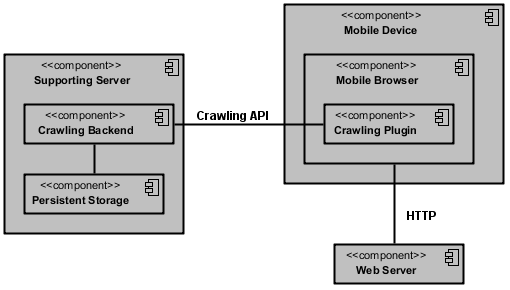
\includegraphics[scale=0.70]{diagrams/component_diagram.png}
\caption{Prototype's Runtime Interactions.}
\label{fig:component_diagram}
\end{figure}


\subsection{Prototype}
We took advantage of the fact that the FourthParty\footnote{http://www.fourthparty.info} project is open-source. After analyzing its codebase, we ported its core functionality over to support Android-based mobile devices, such as smartphones and tablets. FourthPartyMobile is implemented in Java and Javascript, leveraging both the Android SDK and the Mozilla Add-On SDK. Persistent storage is fully compliant with FourthParty's SQLite database schema. Thus, we provide a standardized representation for traditional and mobile crawls, which facilitates data analysis. Our Crawling Backend is written in java with a SQLite JDBC library that supports Mac OS, Linux and Windows, so it should be fully multi-platform. It also supports concurrency, so multiple crawls can be recorded simultaneously. 

\section{Methodology}
DIEGO

\section{Data Analysis}

\subsection{Main Players}
CHRIS

Three types of players: advertisers, content providers, and third-party content providers (embedded in sites)

\subsection{Cookie/Javascript Pervasiveness}
CHRIS

By website category (e.g. porn, news, etc) and by domain (e.g. com, net, etc)

\subsection{Desktop vs Mobile Tracking}
ALL OF US

\subsection{Physical vs Emulated Devices}
DIEGO

\subsection{Privacy Policy Case Study}
After running our web crawls, we designed a case study in which we look at the privacy policies and related data collected from our crawls of three categories of websites that we found were amongst the most popular sites today: social networks, news sites, and e-commerce sites. While pornography sites are also amongst the most popular sites online, we do not include this fourth category in our case study for reasons of decency. 

Based on the list of the Alexa Top 100 US visited websites, we chose three websites amongst the top 25 most visited sites, one representing each of our three categories. Our case study examines the privacy policies of LinkedIn\footnote{http://www.linkedin.com} (social network), CNN\footnote{http://www.cnn.com} (news) and Amazon\footnote{http://www.amazon.com} (e-commerce).

The case study has five stages, each stage looking at the privacy policies in more detail:
\begin{enumerate}
\item Compare the contents of the privacy policies displayed when visiting each of the sites on our three platforms (desktop, tablet, and smartphone).
\item Compare the length of the privacy policies of each website.
\item Examine the topics covered, i.e., the sections included in the policies.
\item Inspect some of the language used in select sections of the policies.
\item Compare the presented cookie policies with the collected web crawl data.
\end{enumerate}

\section{Conclusions and Future Work}

\nocite{*}
\bibliographystyle{abbrv}
\bibliography{sigproc}
\end{document}
